\section{Simulation Analysis}
\label{sec:simulation}


\subsection{1}
%Op_Tab
The results obtained from the simulation are shown in the table below. 

\begin{table}[H] \centering
\begin{tabular}{|
>{\columncolor[HTML]{FFCC67}}l l
>{\columncolor[HTML]{FFCC67}}l l|}
\hline
\cellcolor[HTML]{EABD8B}Name & \cellcolor[HTML]{EABD8B}Value {[}A or V{]} & \cellcolor[HTML]{EABD8B}Name & \cellcolor[HTML]{EABD8B}Value {[}A or V{]} \\ \hline
@gb                          & -2.86455e-04                               & V1                           & 5.216040e+00                                   \\
@R1{[}i{]}                   & 2.732478e-04                               & V2                           & 4.939074e+00                                   \\
@R2{[}i{]}                   & -2.86455e-04                               & V3                           & 4.361415e+00                                   \\
@R3{[}i{]}                   & -1.32073e-05                               & V5                           & 4.978786e+00                                 \\
@R4{[}i{]}                   & 1.229564e-03                               & V6                           & 5.853598e+00                               \\
@R5{[}i{]}                   & 1.316042e-03                               & V7                          & 
-2.00109e+00       \\
@R6{[}i{]}                   & 9.563162e-04                               & V8                           & -2.97875e+00                               \\
@R7{[}i{]}                   & 9.563162e-04                               & V9                           & 
0.000000e+00       \\
 \hline
\end{tabular}
\caption{NgSpice simulation results 1}
\end{table}

\subsection{2}

%Op2_tab
\begin{table}[H] \centering
\begin{tabular}{|
>{\columncolor[HTML]{FFCC67}}l l
>{\columncolor[HTML]{FFCC67}}l l|}
\hline
\cellcolor[HTML]{EABD8B}Name & \cellcolor[HTML]{EABD8B}Value {[}A or V{]} & \cellcolor[HTML]{EABD8B}Name & \cellcolor[HTML]{EABD8B}Value {[}A or V{]} \\ \hline
@gb                          & 0.000000e+00                               & V1                           & 0.000000e+00                                  \\
@R1{[}i{]}                   & 0.000000e+00                               & V2                           & 0.000000e+00                                   \\
@R2{[}i{]}                   & 0.000000e+00                               & V3                           & 0.000000e+00                                   \\
@R3{[}i{]}                   & 0.000000e+00                               & V5                           & 0.000000e+00                                 \\
@R4{[}i{]}                   & 0.000000e+00                               & V6                           & 5.000000e+01                               \\
@R5{[}i{]}                   & -1.63724e-02                               & V7                          & 
0.000000e+00      \\
@R6{[}i{]}                   & 0.000000e+00                               & V8                           & 0.000000e+00                              \\
@R7{[}i{]}                   & 0.000000e+00                               & V9                           & 
0.000000e+00       \\
 \hline
\end{tabular}
\caption{NgSpice simulation results 2}
\end{table}

\subsection{3}

%plot_natural

\begin{figure}[h] \centering

\begin{subfigure}{0.4\textwidth}
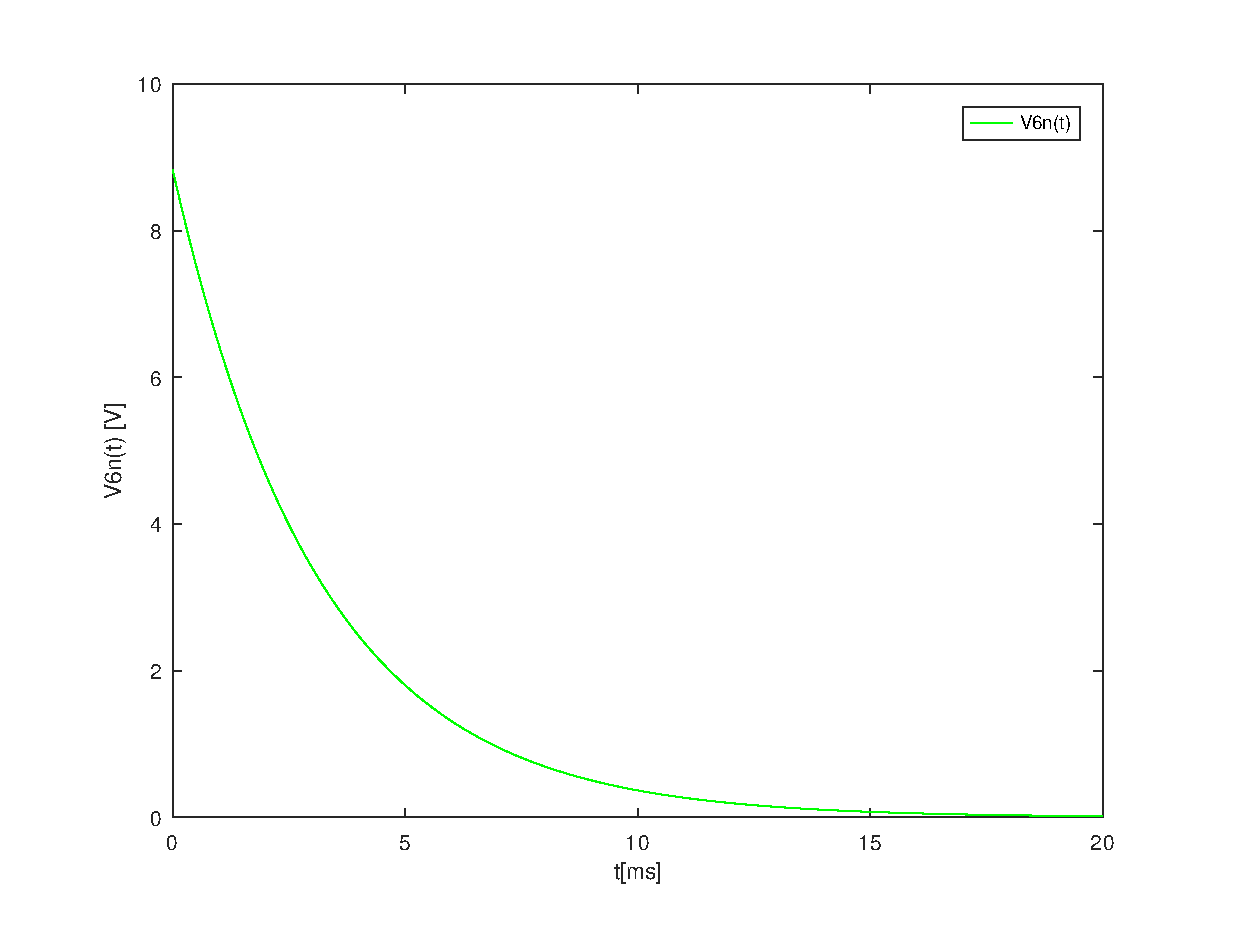
\includegraphics[width=\textwidth]{NaturalResponse.eps}
\caption{Natural Response (Octave)}
\label{fig:first}
\end{subfigure}
\begin{subfigure}{0.4\textwidth}
\includegraphics[width=\textwidth]{sim_3.pdf}
\caption{Natural Response (NGSpice)}
\label{fig:second}
\end{subfigure}

\end{figure}

%se for preciso
%\end{figure}
%\begin{figure}[H]
%\centering
%\includegraphics[width = 15cm]{sim_3.pdf}
%\caption {Ngspice simulation plot 1}
%\end{figure}

\subsection{4}	

\begin{figure}[h] \centering

\begin{subfigure}{0.4\textwidth}
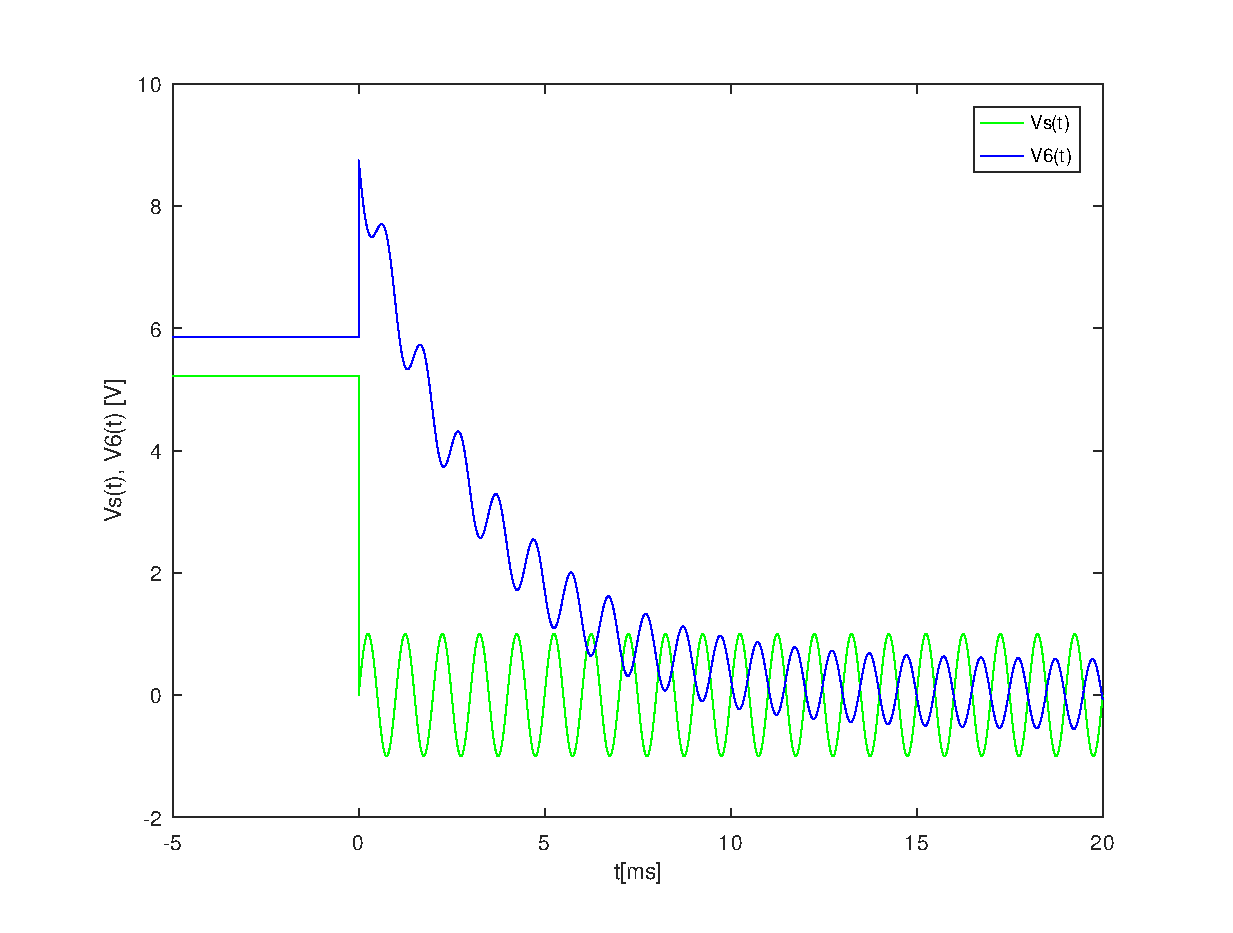
\includegraphics[width=\textwidth]{Solution.eps}
\caption{Natural and forced response (Octave)}
\label{fig:first}
\end{subfigure}
\begin{subfigure}{0.4\textwidth}
\includegraphics[width=\textwidth]{sim4.pdf}
\caption{Natural and forced response}
\label{fig:second}
\end{subfigure}

\end{figure}

%se for preciso
%\begin{figure}[H]
%\centering
%\includegraphics[width = 15cm]{sim4.pdf}
%\caption {Ngspice simulation plot 2}
%\end{figure}

\subsection{5}

\begin{figure}[h] \centering

\begin{subfigure}{0.4\textwidth}
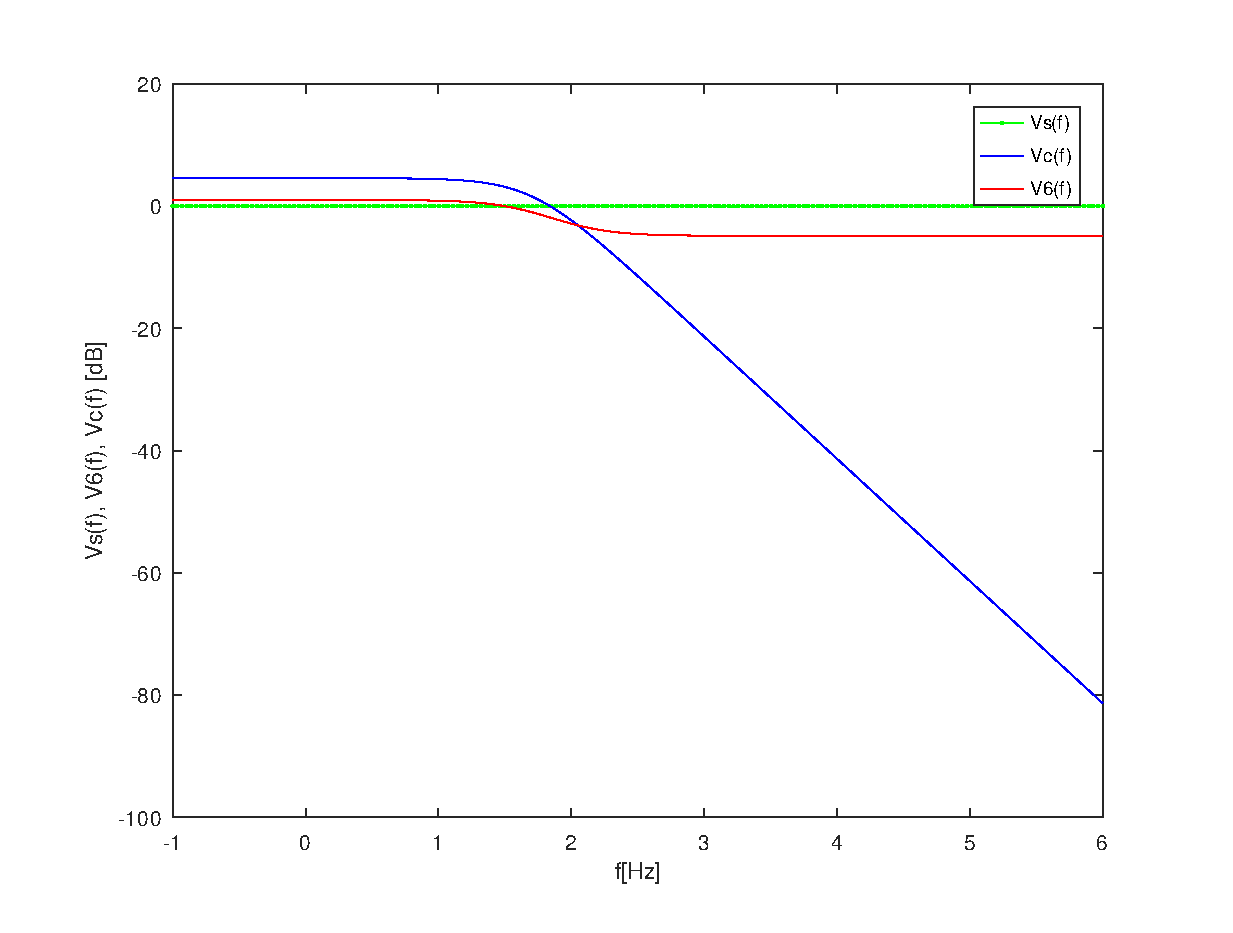
\includegraphics[width=\textwidth]{Amplitude.eps}
\caption{First Circuit}
\label{fig:first}
\end{subfigure}
\begin{subfigure}{0.4\textwidth}
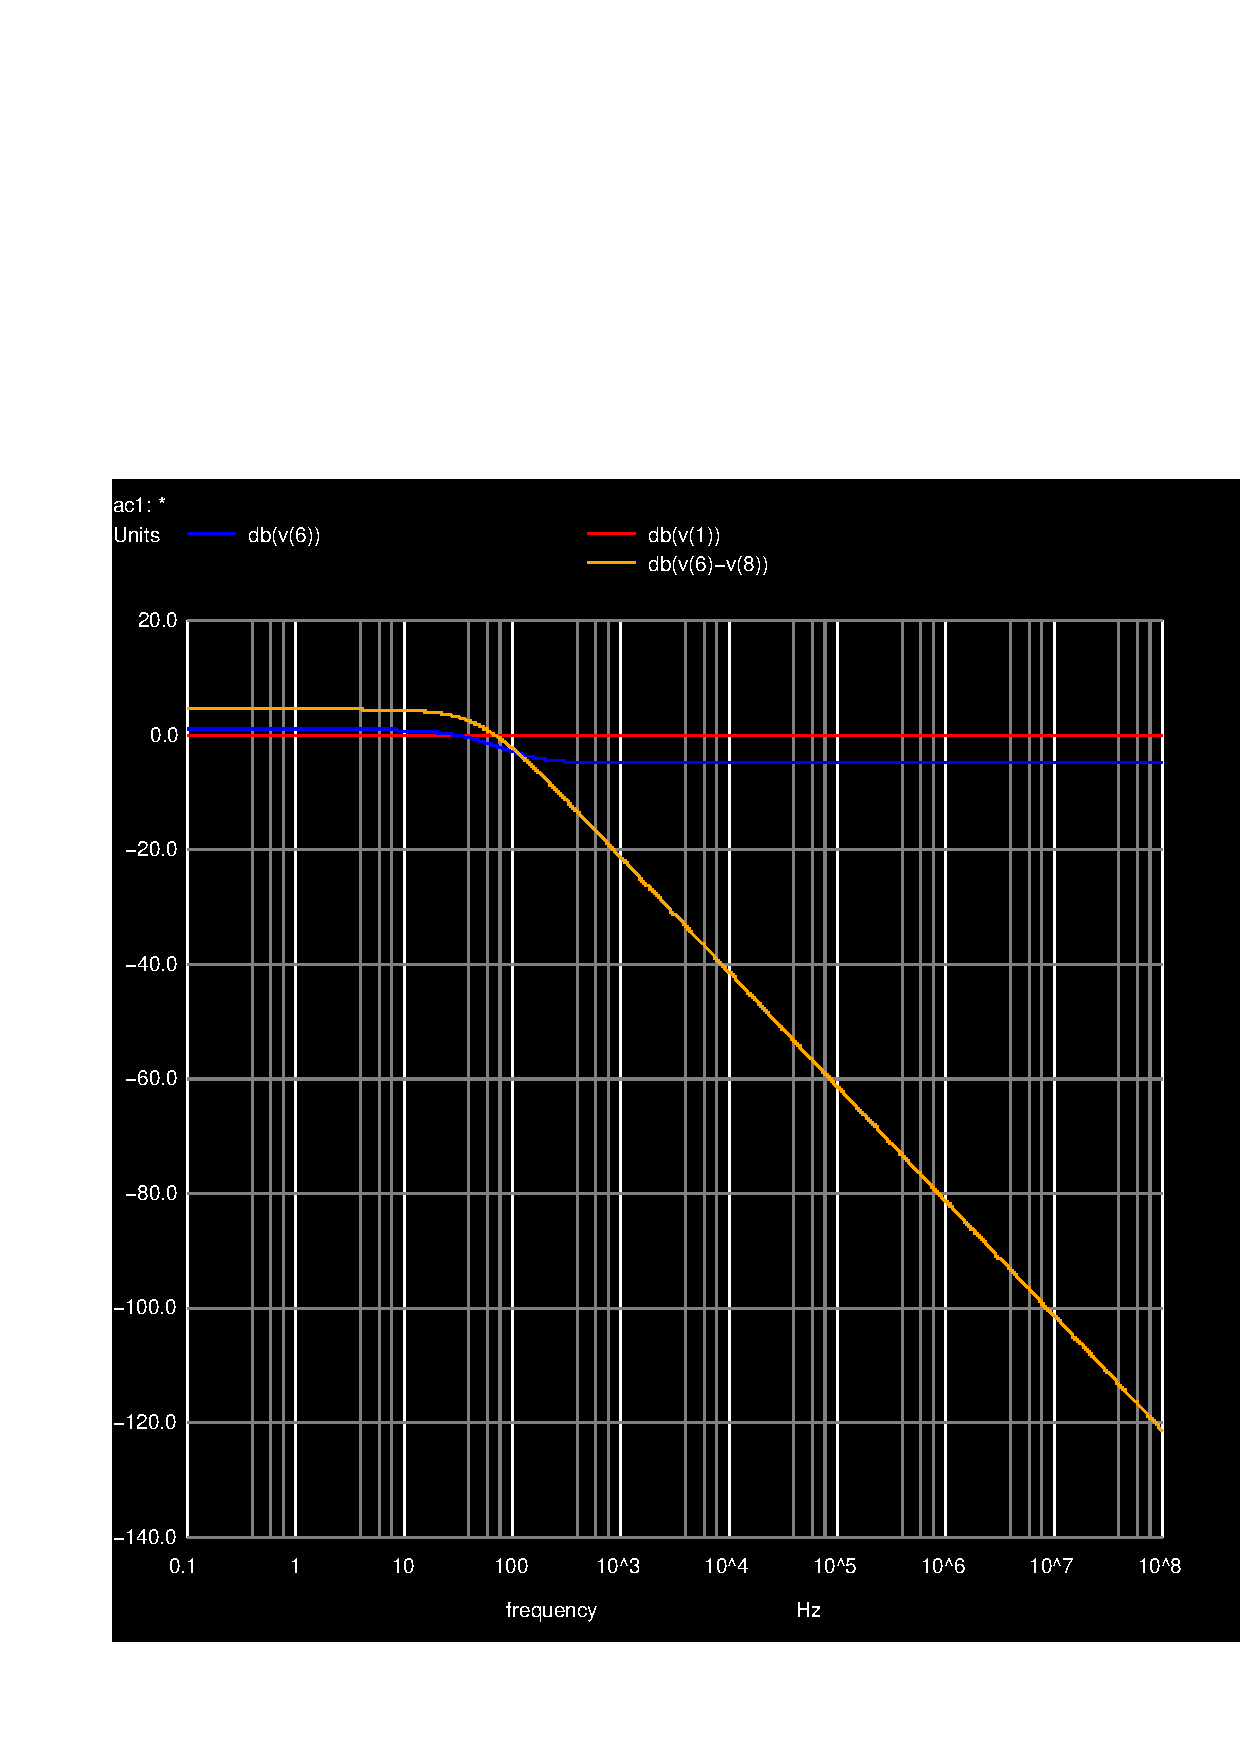
\includegraphics[width=\textwidth]{sim5_db.pdf}
\caption{Second Circuit}
\label{fig:second}
\end{subfigure}

\end{figure}


%se for preciso
%\begin{figure}[H]
%\centering
%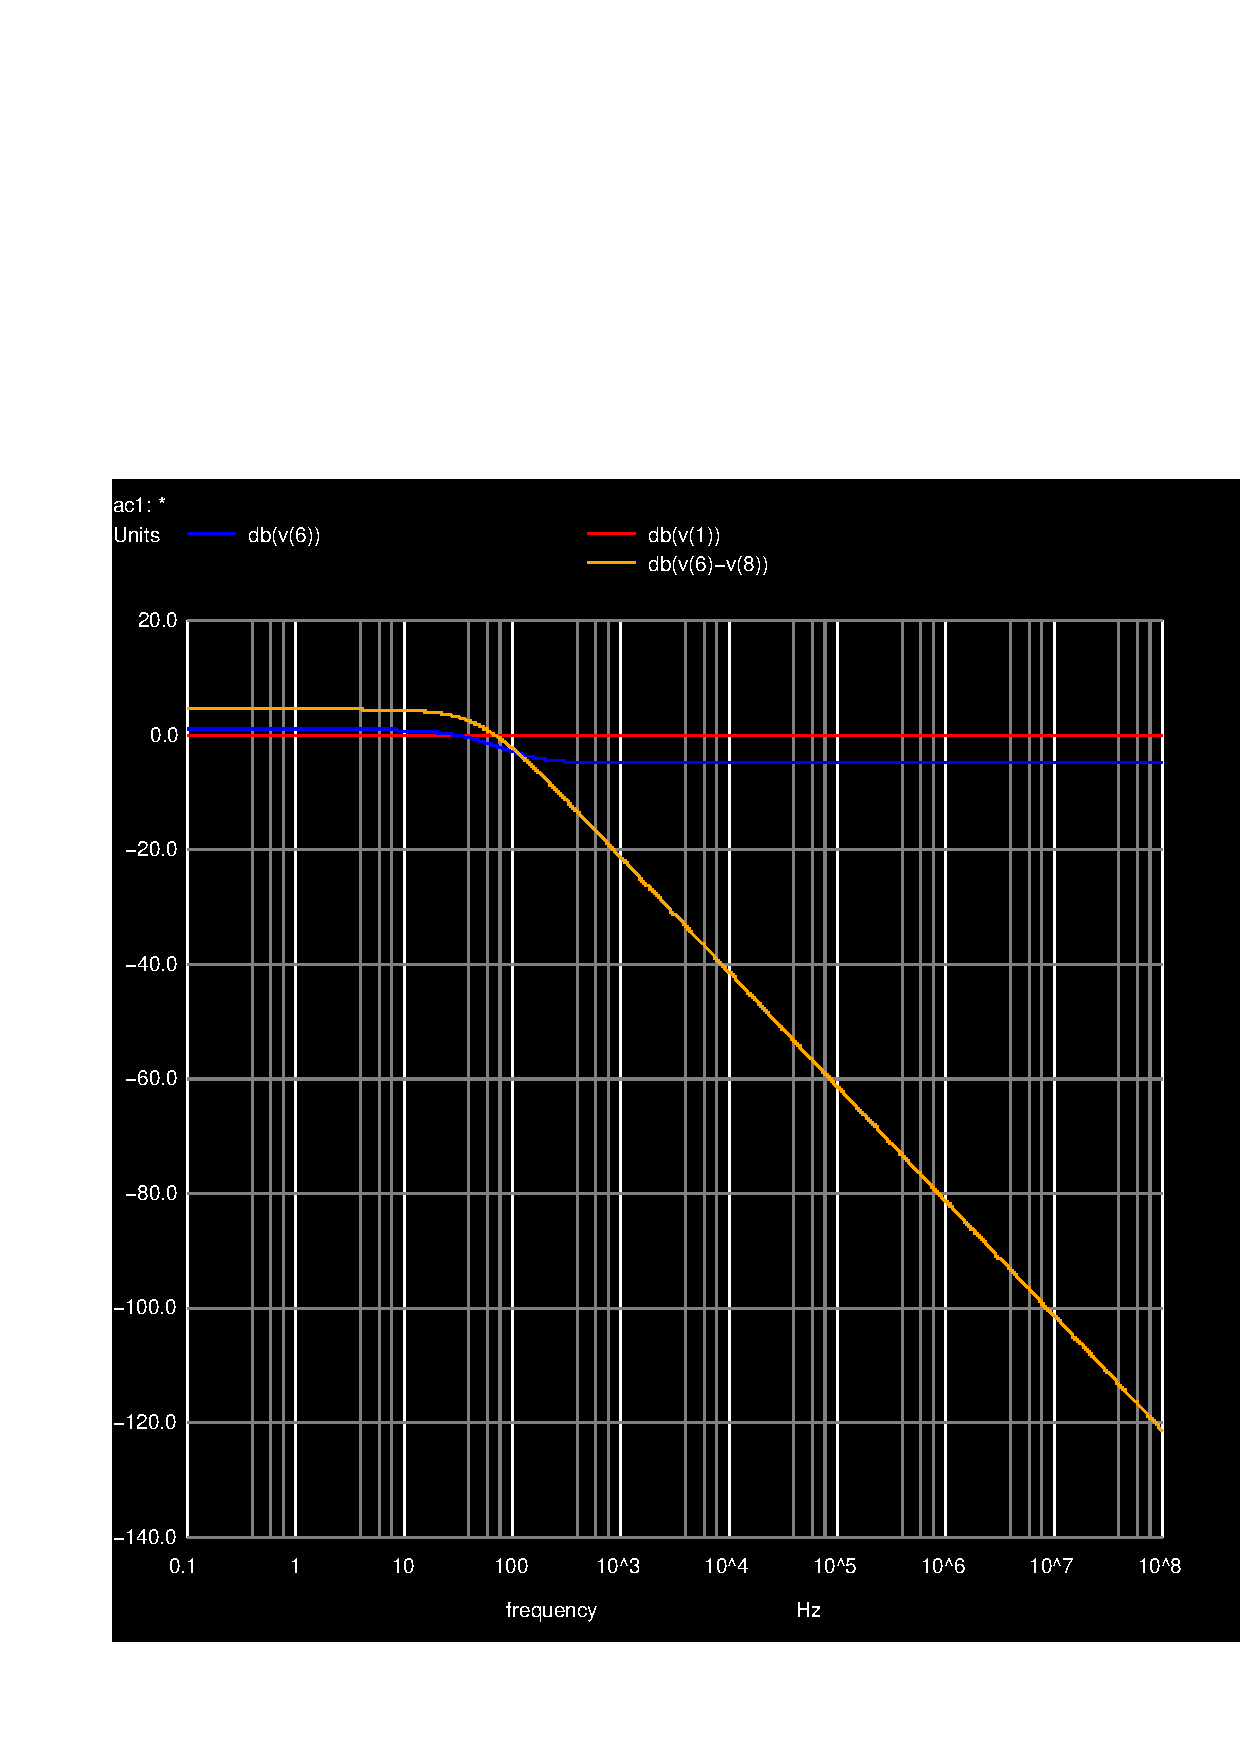
\includegraphics[width = 15cm]{sim5_db.pdf}
%\caption {Ngspice simulation plot 3}
%\end{figure}


\begin{figure}[h] \centering

\begin{subfigure}{0.4\textwidth}
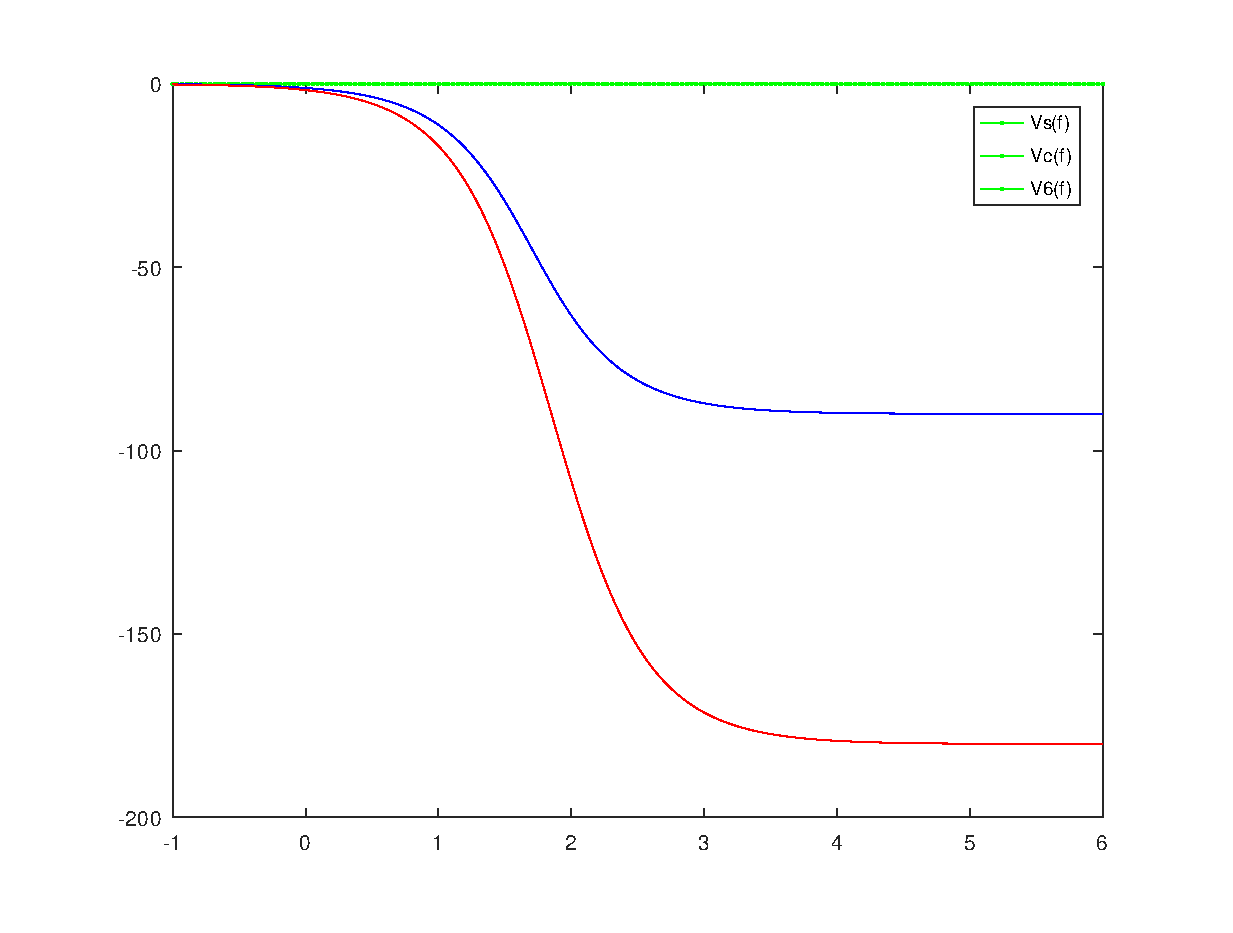
\includegraphics[width=\textwidth]{Arguments.eps}
\caption{First Circuit}
\label{fig:first}
\end{subfigure}
\begin{subfigure}{0.4\textwidth}
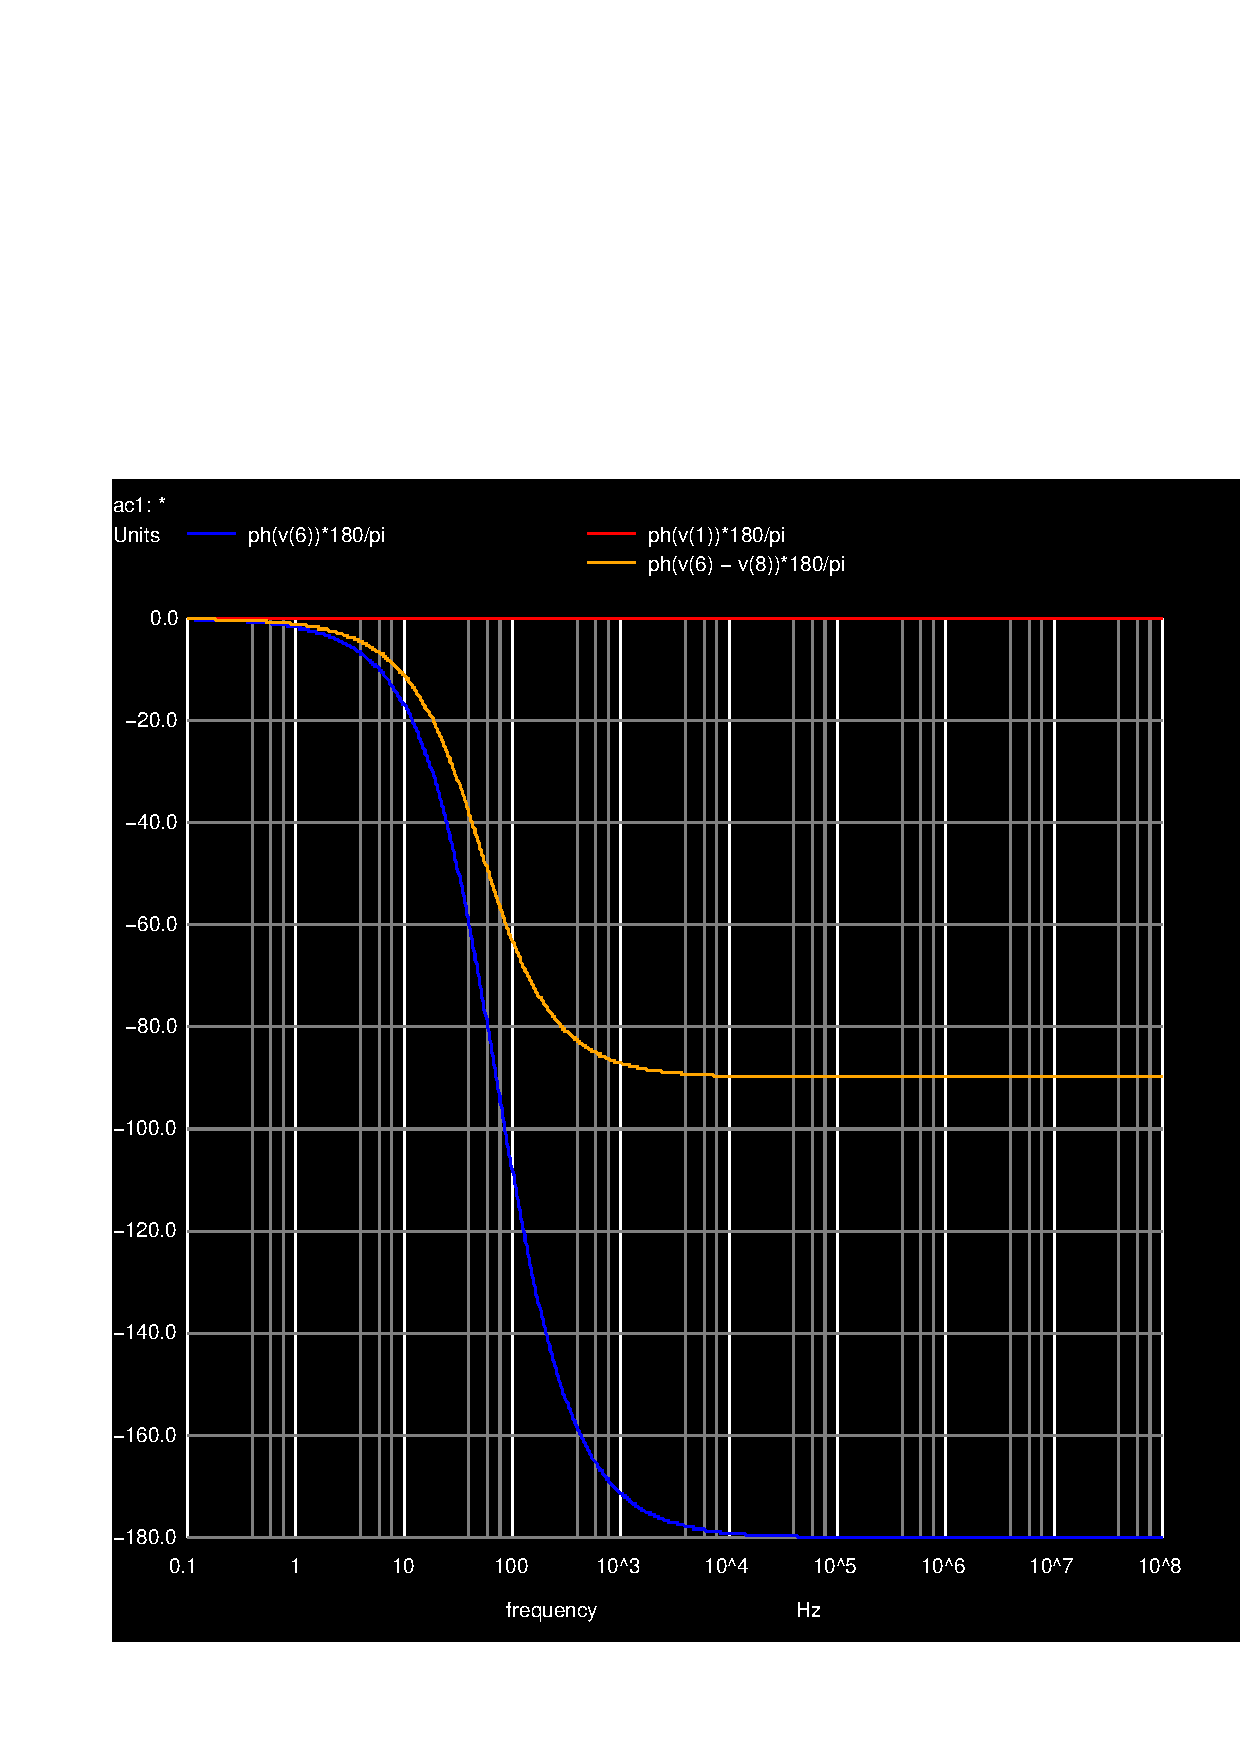
\includegraphics[width=\textwidth]{sim5_ph.pdf}
\caption{Second Circuit}
\label{fig:second}
\end{subfigure}

\end{figure}


%se for preciso
%\begin{figure}[H]
%\centering
%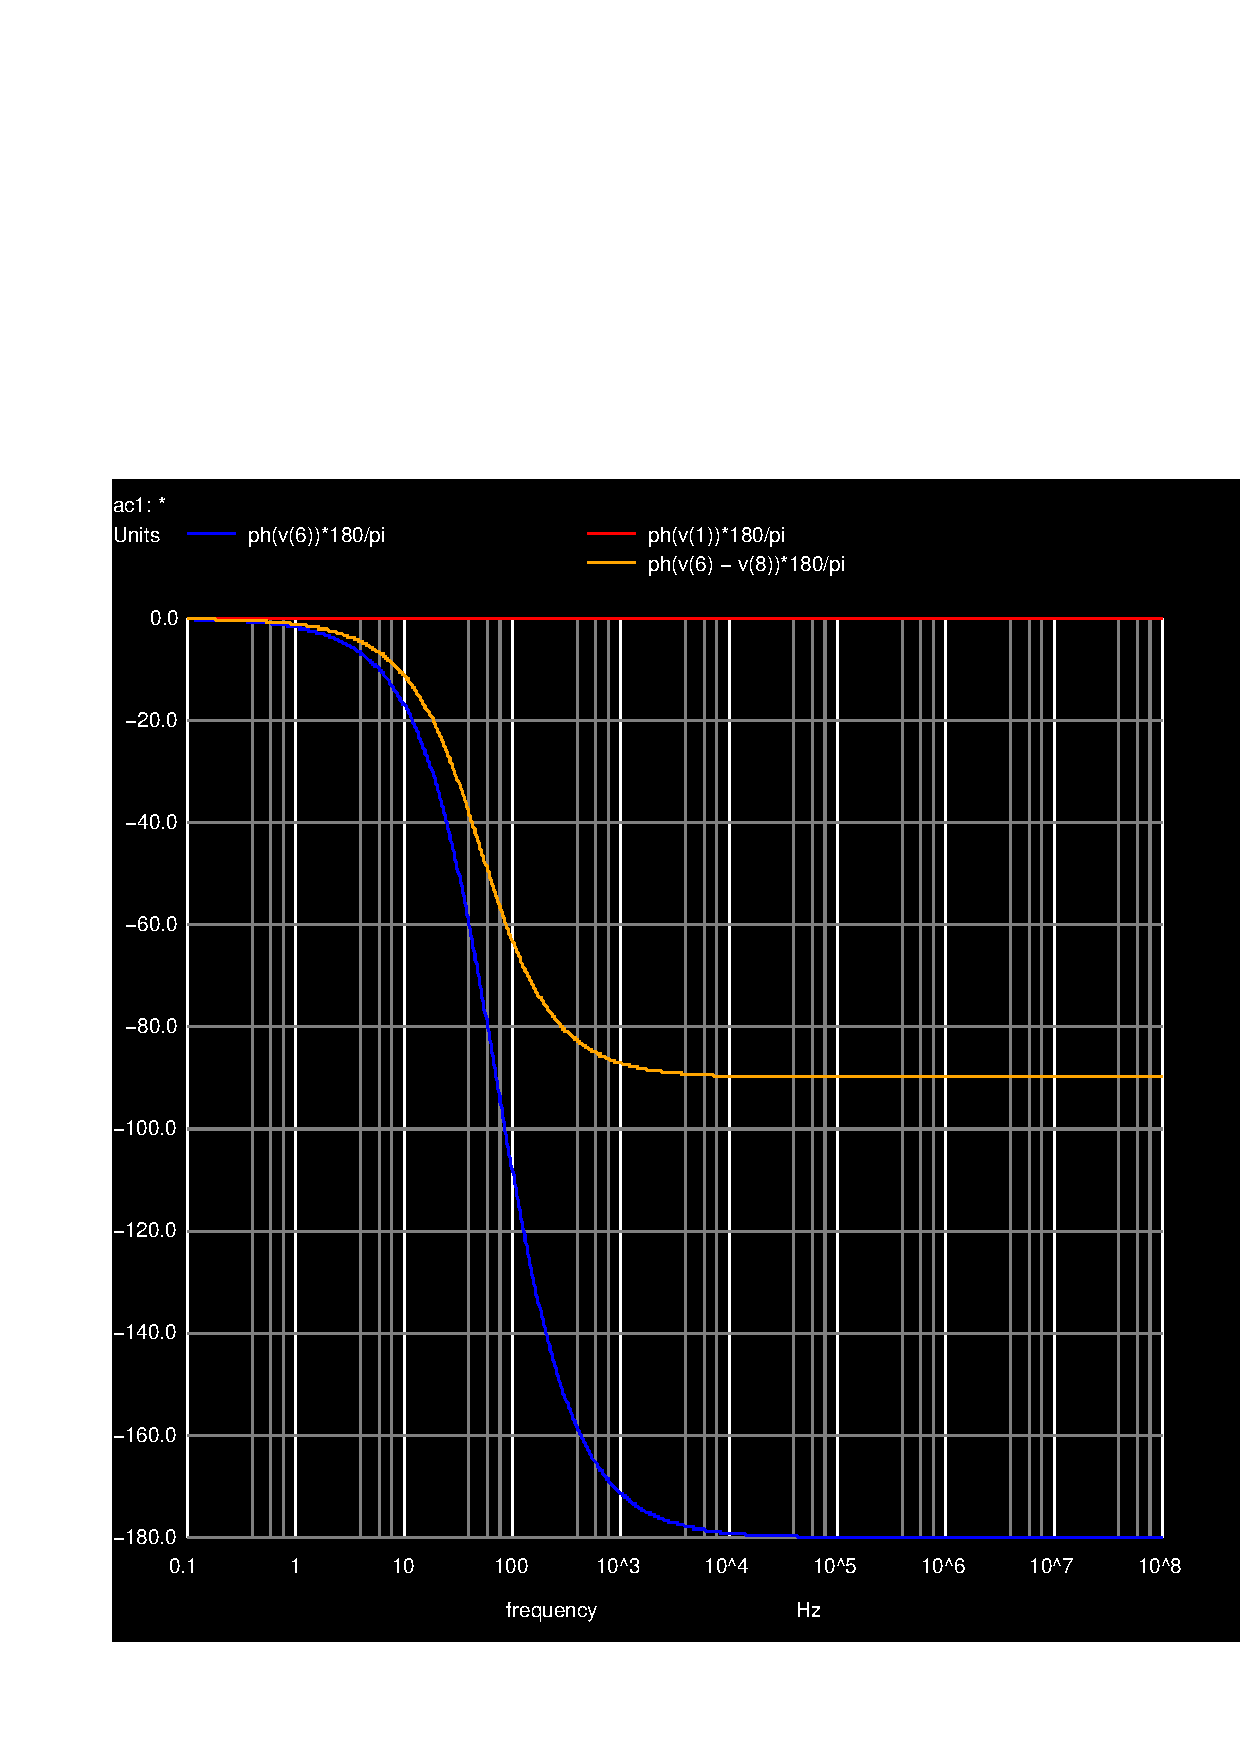
\includegraphics[width = 15cm]{sim5_ph.pdf}
%\caption {Ngspice simulation plot 4}
%\end{figure}

